% !Mode:: "TeX:UTF-8"
%% This is file `mcmthesis-demo.tex',
%% generated with the docstrip utility.
%%
%% The original source files were:
%%
%% mcmthesis.dtx  (with options: `demo')
%%
%% -----------------------------------
%%
%% This is a generated file.
%%
%% Copyright (C)
%%     2010 -- 2015 by Zhaoli Wang
%%     2014 -- 2016 by Liam Huang
%%     2017         by Zhuang Ma
%%     2018美赛,为了迈思数模内部学员更快的掌握CTEX,由迈思数模站长对本模板进行调整
%% This work may be distributed and/or modified under the
%% conditions of the LaTeX Project Public License, either version 1.3
%% of this license or (at your option) any later version.
%% The latest version of this license is in
%%   http://www.latex-project.org/lppl.txt
%% and version 1.3 or later is part of all distributions of LaTeX
%% version 2005/12/01 or later.
%%
%% This work has the LPPL maintenance status `maintained'.
%%
%% The Current Maintainer of this work is Liam Huang.
%% 上述内容为介绍改模板的背景

\documentclass{mcmthesis}
\mcmsetup{CTeX = true,   % 使用 CTeX 套装时,设置为 true
        tcn = 84018, problem = C,
        sheet = true, titleinsheet = true, keywordsinsheet = true,
        titlepage = true, abstract = false}
%设置摘要页格式,一般按照该设置就行,true表示选择,false表示不选择,需要修改控制号和选择的题目
\usepackage{palatino}
\usepackage[section]{placeins}
%\usepackage{lipsum} %添加lipsum宏包,就是随机生成一段文本,可以不使用

\usepackage[UTF8, nocap]{ctex} %如果想使用中文输入的话,可以增加该宏包
\usepackage{amsmath}

\title{We Will Get O Prize(Not U Prize)}
%\author{\small \href{http://www.latexstudio.net/}
% {
\includegraphics[width=7cm]{mcmthesis-logo}}}
%\date{\today}

%正文摘要和控制页摘要名字修改
%\def\abstractname{Abstract}
%\def\sheetsummaryname{Summary}
\tolerance=1
\emergencystretch=\maxdimen
\hyphenpenalty=10000
\hbadness=10000


\begin{document}

 %控制页摘要内容
\begin{sheetsummary}
%\lipsum[1]
%lipsum是显示一段无意义的文字
%Ru guo ni bu xiang xian shi zhe duan wen zi, qing ba \textit{lipsum} shanchu.\\
%如果你不想显示上面的那段文字,那就把 \textit{lipsum}删掉
%获得更多的latex教材,请添加latex交流群,或者关注迈思数模微信公众号:shumohome
%并回复“LATEX资料”
%美赛LATEX模板交流群:193607493
hello world
\end{sheetsummary}

% %正文摘要内容
%\begin{abstract}
%\lipsum[2]
%\end{abstract}

%关键词
\begin{keywords}
hello; world
\end{keywords}

\maketitle
 % Generate the Table of Contents, if it's needed.
\tableofcontents
\newpage

\section{Overview}
    \subsection{Background}
    The rapid development of modern social economy benefits from the development of energy production. The issue of energy usage and production has always been the focus of world economic development.

    In the 21st century, with the economic development and improvement, the energy shortage and the increasing contradiction between supply and demand. Meanwhile, the production and use of fossil energy sources have had a huge negative impact on the environment. Therefore, developing clean and renewable energy is imperative.

    The differences between states such as geography, industry, population, climate lead to the contradiction of energy supply.
    Interstate cooperation and joint management and development of clean and renewable energy are regarded as the best solution to these problems. Nowadays four state governors  – California, Arizona, New Mexico and Texas  –  wish to form a realistic new energy compact. Texas leads the country in total (non-hydro) installed renewable energy capacity, almost all of which comes from the state’s 9,410 MW of wind capacity. California is the leader in solar energy installed capacity, both for photovoltaic technology (738 MW) and concentrating solar power (364 MW).

    \subsection{Restatement of the Problem}
    We are required to provide an overview of energy profile for each of the four states and model how these profiles have evolved from 1960 to 2009. In addition, it is necessary to make our results understandable through discussion, including similarities and differences between 4 states. Then we need to establish a criteria model and choose the "best" profile use of cleaner, renewable energy usage targets. Finally, we need to give our suggestions about exact action to achieve the goal we set based on what we predict.

    In order to identify
    In order to determine whether it is clean and renewable energy, for which we check the information and classification of various types of energy.


    \noindent
    cleaner, renewable energy ( defination from SEDS and ):
    \begin{itemize}
      \item Conventional hydroelectric power
      \item Solar thermal direct use energy and photovoltaic electricity net generation
      \item Electricity produced by wind
      \item Wood and wood-derived fuels, biomass waste
      \item Fuel ethanol minus denaturant
    \end{itemize}

\section{Notations and Assumptions}

    \subsection{Notations}
         \begin{table}[!htbp]
           %\centering
                \begin{tabular}{c|l}
                  \hline
                  Symbol & Meaning \\
                  \hline
                  n & the number of samples \\
                  p & the number of original indicators \\
                  k & the number of principal component \\
                  X & \{$x_{ij}$\} original data matrix (i = 1, 2,…, n ; j = 1,2,…,p ) \\
                  Z & \{$z_{ij}$\} standardization matrix with z-scores (i = 1, 2,…, n ; j = 1,2,…,p ) \\
                  U & \{$u_{ij}$\} partial covariance matrix (i = 1, 2,…, n ; j = 1,2,…,p ) \\
                  C & \{$c_{ij}$\} covariance matrix (j = 1,2,…,p ) \\
                  R & \{$r_{ij}$\} correlation matrix (j = 1,2,…,p ) \\
                  F & \{$f_{ij}$\} The eigenvectors matrix of Z (j = 1,2,…,p ) \\
                  Y & \{$y_{ij}$\} principal component matrix (i = 1, 2,…, n ; j = 1,2,…,k) \\
                  V & \{$v_{ij}$\} decision matrix (i = 1, 2,…, n ; j = 1,2,…,k) \\
                  $A^+$/$A^-$ & positive / negative ideal profile \\
                  $S_{i}^+$/$S_{i}^-$ & positive / negative ideal profile \\
                  $\lambda_{j}$ & the eigenvalues of Z (j=1,2,…,p) \\
                  $y_{i}$ & principal component \\
                  $C_{i}$ & the final performance score in TOPSIS method \\
                  kmo & the value of KMO test \\
                  \hline
                \end{tabular}
           \caption{Abbreviation and Description}
         \end{table}

    \subsection{Assumptions and Justifications}
        \noindent
        We make the following basic assumptions in order to simplify the problem. Each of our assumptions is justified and is consistent with the basic fact.
        \begin{enumerate}
          \item \textbf{Ignore the external costs caused by power generation other than coal:}

              In 2005, the mean external damage of coal in the United States due to coal combustion was 3.2 cents/kWh, The external cost of natural gas power generation is 0.16 cents/kwh, which is actually almost entirely caused by coal-fired power. Also life-cycle CO2 emissions from nuclear, wind, biomass, and solar appear so small as to be negligible compared with those from fossil fuels.(information comes from the report "Hidden cost of energy unpriced consequences of energy production and use" )
          \item \textbf{The conversion between generation and consumption is 100\%, and the consumption is used to represent the amount of power generation to evaluate.}

        \end{enumerate}


\section{Model overview}
    Firstly, considering energy production and consumption, environmental impact, technology, economy, we extract 12 variables from 605 variables to get general energy profile of each state.

    In order to show the evolution of energy production, we construct a comprehensive evaluation index system for the level of cleaner, renewable energy development. We use the \textbf{Principal Component Analysis} method to carry out the correlation cluster analysis of the index. To make the similarities and differences between 4 states understandable, we use \textbf{TOPSIS} method to show our results.At the same time, we can get the extracted principal componment choosing the "best" profile from comprehensive evaluation results ranking.

    After determining the “best” profile, we use \textbf{ARIMA} method to predict the energy profile of each state, especially as we evaluate the cleaner, renewable energy development in the future.



        \begin{enumerate}
          \item There are three options for each vehicle arriving at the toll plaza and each car entered the shortest path of the queue.
          \item All the toll booths are same except charge method (width, construction cost e.t.c )
          \item The arrival process is Poisson
        \end{enumerate}


\section{Statement of our Model}

    \subsection{Definition}
        \begin{table}
          \centering
                \begin{tabular}{ll}
                \hline
                h  &  Conventional (human-staffed) tollbooths \\
                a  &  Exact-change (automated) tollbooths \\
                e  &  Electronic toll collection booths \\
                B$_{i}$  &  Number of types i tollbooths \\
                b$_{i}$  &  Number of type i tollbooths to open, where a \\
                B  &  Number of tollbooths \\
                L  &  Number of main lanes \\
                l$_{i}$  &  Lower bound for the number of type i lanes to open \\
                u$_{i}$  &  Upper bound for the number of type i lanes to open \\
                $\lambda _{i}$ & Mean arrival rate for lane type i, where \\
                \hline
                \end{tabular}
            \caption{Definition}
        \end{table}

        \begin{itemize}
              \item h--Conventional (human-staffed) tollbooths
              \item a--Exact-change (automated) tollbooths
              \item e--Electronic toll collection booths
              \item B$_{i}$--Number of types i tollbooths
              \item b$_{i}$--Number of type i tollbooths to open, where
              \item B--Number of tollbooths
              \item L--Number of main lanes
              \item l$_{i}$--Lower bound for the number of type i lanes to open
              \item u$_{i}$--Upper bound for the number of type i lanes to open
              \item $\lambda_{i}$--Mean arrival rate for lane type i, where
              \item $\lambda$--Mean total arrival rate of vehicles at the toll plaza, i.e., the number of arrivals per unit time
              \item $\mu_{i}$--Mean service rate for a type i tollbooth, i.e., the number of service completions per unit time
              \item $\sigma_{i}$--Standard deviation of service time for a type i tollbooth
              \item W--Mean total waiting time in the queue for all arrivals at the toll plaza
              \item c$_{i}$--The rate of the operating cost of a type i lane
              \item d--The rate of the operating cost of a type i lane
              \item c$_{o}$--The total operating costs at the toll plaza per unit time
              \item c$_{w}$--The total user-waiting costs at the toll plaza per unit time
              \item Z--The sum of total operating and user-waiting costs at the toll plaza per unit time
              \item l--the length of buffer segment
              \item w--the width of booth
              \item y$_{i}$--Traffic accident prediction
        \end{itemize}










    \begin{itemize}
    \item minimizes the discomfort to the hands, or
    \item maximizes the outgoing velocity of the ball.
    \end{itemize}
    We focus exclusively on the second definition.

    \begin{itemize}
    \item the initial velocity and rotation of the ball,
    \item the initial velocity and rotation of the bat,
    \item the relative position and orientation of the bat and ball, and
    \item the force over time that the hitter hands applies on the handle.
    \end{itemize}
    \begin{itemize}
    \item the angular velocity of the bat,
    \item the velocity of the ball, and
    \item the position of impact along the bat.
    \end{itemize}
    \emph{center of percussion} [Brody 1986],

    \begin{Theorem} \label{thm:latex}
    \LaTeX
    \end{Theorem}
    \begin{Lemma} \label{thm:tex}
    \TeX .
    \end{Lemma}
    \begin{proof}
    The proof of theorem.
    \end{proof}

    \subsection{Other Assumptions}

    \begin{itemize}
    \item
    \item
    \item
    \item
    \end{itemize}



\section{Analysis of the Problem}
\begin{figure}[h]
%\small
\centering
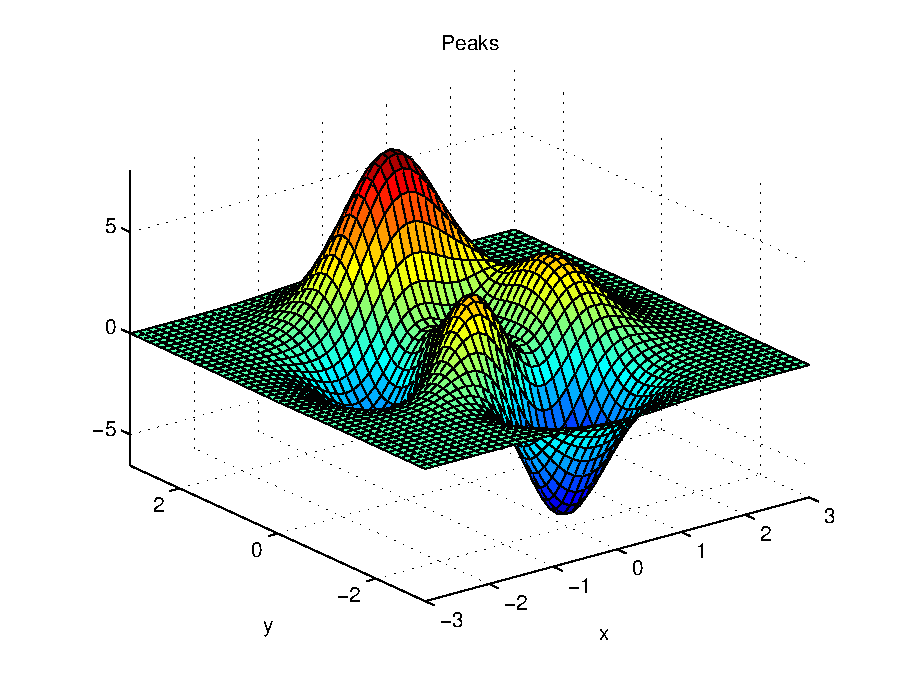
\includegraphics[width=12cm]{mcmthesis-aaa.eps}
\caption{Figure example 1} \label{fig:aa}
\end{figure}


Figure \ref{aa}.

\begin{figure}[h]
\begin{minipage}[h]{0.5\linewidth}
\centering

\includegraphics[width=0.8\textwidth]{0.jpg}
\caption{Figure example 2}
\end{minipage}
\begin{minipage}[h]{0.5\linewidth}
\centering

\includegraphics[width=0.8\textwidth]{0.jpg}
\caption{Figure example 3}
\end{minipage}
\end{figure}



\begin{equation}
a^2 \label{aa}
\end{equation}

\[
  \begin{pmatrix}{*{20}c}
  {a_{11} } & {a_{12} } & {a_{13} }  \\
  {a_{21} } & {a_{22} } & {a_{23} }  \\
  {a_{31} } & {a_{32} } & {a_{33} }  \\
  \end{pmatrix}
  = \frac{{Opposite}}{{Hypotenuse}}\cos ^{ - 1} \theta \arcsin \theta
\]


\[
  p_{j}=\begin{cases} 0,&\text{if $j$ is odd}\\
  r!\,(-1)^{j/2},&\text{if $j$ is even}
  \end{cases}
\]



\[
  \arcsin \theta  =
  \mathop{{\int\!\!\!\!\!\int\!\!\!\!\!\int}\mkern-31.2mu
  \bigodot}\limits_\varphi
  {\mathop {\lim }\limits_{x \to \infty } \frac{{n!}}{{r!\left( {n - r}
  \right)!}}} \eqno (1)
\]

\section{Calculating and Simplifying the Model  }


$\mathop{A}_{ij}$ and $A_{ij}$ 不一样

$\left(123 \right)$ and $(123)$ and (123) 不一样
\section{The Model Results}


\section{Validating the Model}

CTEX中最繁琐的是表格输入,不过数学建模竞赛中,一般要求输入三线表,这样统一格式的情况下,对于输入表格就简单一点了。\\
\\
双斜杠是强制换行,在矩阵,表格,大括号的公式常用。\\
关于表格的合并,见下一部分。给出的例子。
\begin{center}
\begin{tabular}{c|cclcrcc}
\hline
Year & theta & $S_1^-$ & $S_2^-$ & $S_3^-$ & $S_4^+$ & $S_5^+$ & $S_6^+$ \\%表格标题
\hline
2016 & 1      & 0      & 0 & 0.0001 & 0      & 0      & 0 \\
2017 & 0.9997 & 0.0555 & 0 & 0.2889 & 0.1844 & 0.463  & 0 \\
2018 & 0.9994 & 0      & 0 & 0.0012 & 0.3269 & 0.7154 & 0 \\
2019 & 0.9993 & 0      & 0 & 0      & 0.4325 & 1.0473 & 0 \\
2020 & 0.9991 & 0      & 0 & 0      & 0.5046 & 1.2022 & 0 \\
2021 & 0.999  & 0      & 0 & 0      & 0.5466 & 1.2827 & 0 \\
2022 & 0.9989 & 0.0017 & 0 & 0.3159 & 0.562  & 1.2995 & 0 \\
2023 & 0.9989 & 0      & 0 & 0.0109 & 0.5533 & 1.2616 & 0 \\
2024 & 0.9989 & 0      & 0 & 0      & 0.5232 & 1.1769 & 0 \\
2025 & 0.9989 & 0      & 0 & 0.1009 & 0.4738 & 1.0521 & 0 \\
2026 & 0.9991 & 0      & 0 & 0      & 0.4071 & 0.8929 & 0 \\
2027 & 0.9992 & 0.0004 & 0 & 0.1195 & 0.3248 & 0.7042 & 0 \\
2028 & 0.9994 & 0.0164 & 0 & 0.046  & 0.2287 & 0.4902 & 0 \\
2029 & 0.9997 & 0      & 0 & 0.0609 & 0.12   & 0.2545 & 0 \\
2030 & 1      & 0      & 0 & 0      & 0      & 0      & 0 \\
\hline
\end{tabular}
\end{center}

\section{Conclusions}


\begin{center}
\begin{tabular}{c|cc}
\hline
年份 & \multicolumn{2}{c}{指标}\\
\hline
2017 & 0.9997 & 0.0555 \\
2018 & 0.9994 & 0      \\
2019 & 0.9993 & 0      \\
\hline
\end{tabular}
\end{center}


\begin{table}[h]
  \centering
  \begin{tabular}{c|cc}
\hline
年份 & \multicolumn{2}{c}{指标}\\
\hline
2017 & 0.9997 & 0.0555 \\
2018 & 0.9994 & 0      \\
2019 & 0.9993 & 0      \\
\hline
\end{tabular}
  \caption{NAME}\label{SIGN}
\end{table}

Let's to see Table \ref{SIGN}.


\begin{minipage}{0.5\linewidth}
\begin{tabular}{|c|c|c|}
\hline
\multicolumn{2}{|c|}{\multirow{2}{*}{合并}}&测试\\
\cline{3-3}
\multicolumn{2}{|c|}{}& 0.9997  \\
\hline
2019 & 0.9993 & 0 \\
\hline
\end{tabular}
\end{minipage}
\begin{minipage}{0.5\linewidth}
\begin{tabular}{c|ccc}
\hline
年份 & \multicolumn{3}{c}{指标}\\
\hline
\multirow{3}{*}{合并}&2017 & 0.9997 & 0.0555 \\
&2018 & 0.9994 & 0      \\
&2019 & 0.9993 & 0      \\
\hline
\end{tabular}
\end{minipage}





\section{A Summary}


写入你的中文
如果你不想显示上面的那段文字,那就把lipsum删掉

获得更多的latex教材,请添加latex交流群,或者关注迈思数模微信公众号:shumohome
并回复“LATEX资料”
美赛LATEX模板交流群:193607493
美赛LATEX模板交流群:193607493

\section{Evaluate of the Mode}

美赛获得更多的latex教材,请添加latex交流群,或者关注迈思数模微信公众号:shumohome
并回复“LATEX资料”
美赛LATEX模板交流群:193607493
\section{Strengths and weaknesses}

获得更多的latex教材,请添加latex交流群,或者关注迈思数模微信公众号:shumohome
并回复“LATEX资料”
美赛LATEX模板交流群:193607493

\subsection{Strengths}
\begin{itemize}
\item \textbf{Applies widely}\\
This  system can be used for many types of airplanes, and it also
solves the interference during  the procedure of the boarding
airplane,as described above we can get to the  optimization
boarding time.We also know that all the service is automate.
\item \textbf{Improve the quality of the airport service}\\
Balancing the cost of the cost and the benefit, it will bring in
more convenient  for airport and passengers.It also saves many
human resources for the airline. \item \textbf{}
\end{itemize}

\begin{thebibliography}{99}
\bibitem{1} D.~E. KNUTH   The \TeX{}book  the American
Mathematical Society and Addison-Wesley
Publishing Company , 1984-1986.
\bibitem{2}Lamport, Leslie,  \LaTeX{}: `` A Document Preparation System '',
Addison-Wesley Publishing Company, 1986.
\bibitem{3}\url{http://www.latexstudio.net/}
\bibitem{4}\url{http://www.chinatex.org/}
\end{thebibliography}

\begin{appendices}

\section{First appendix}



Here are simulation programmes we used in our model as follow.\\

\textbf{\textcolor[rgb]{0.98,0.00,0.00}{Input matlab source:}}
\lstinputlisting[language=Matlab]{./code/mcmthesis-matlab1.m}

\section{Second appendix}

some more text \textcolor[rgb]{0.98,0.00,0.00}{\textbf{Input C++ source:}}
\lstinputlisting[language=C++]{./code/mcmthesis-sudoku.cpp}

\end{appendices}
\end{document}

%%
%% This work consists of these files mcmthesis.dtx,
%%                                   figures/ and
%%                                   code/,
%% and the derived files             mcmthesis.cls,
%%                                   mcmthesis-demo.tex,
%%                                   README,
%%                                   LICENSE,
%%                                   mcmthesis.pdf and
%%                                   mcmthesis-demo.pdf.
%%
%% End of file `mcmthesis-demo.tex'.
